\chapter{設計と実装}
\label{chap:implementation}

本章では、本研究において実装したESP32上で動作するプログラムの実装の構成を示す。

\section{全体の構成}

本実装は、プラットフォーム非依存な形で実装したWebAssembly実行環境(libwasm)と、
libwasmが提供する機能を呼び出すESP32用のプログラム(ホストプログラム)によりなる。

構成の概観を図\ref{fig:esp32_libwasm}に示した。

\begin{figure}[htbp]
  \caption{本実装の構成}
  \label{fig:esp32_libwasm}
  \begin{center}
    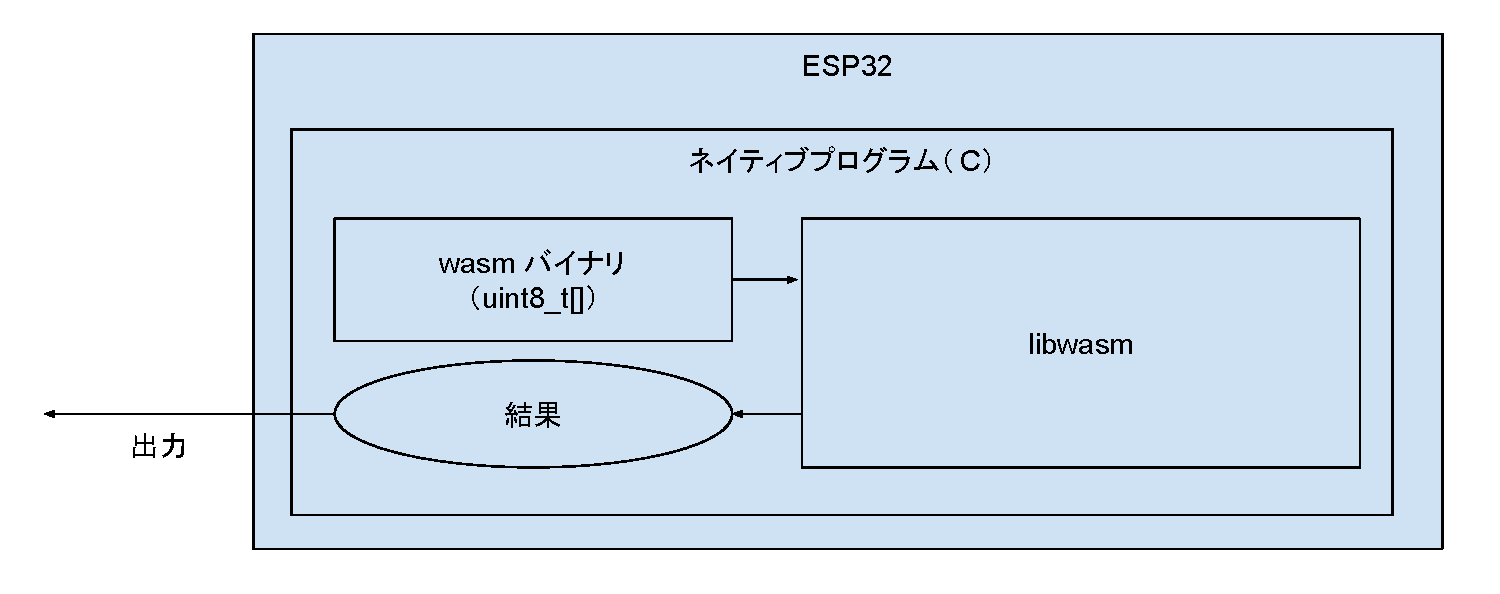
\includegraphics[bb=0 0 800 300,width=12cm]{img/esp32_libwasm.pdf}
  \end{center}
\end{figure}

\section{ホストプログラム}

ホストプログラムは、Espressif Systemsが提供するESP32用ソフトウェア開発環境であるESP-IDF\cite{esp_idf}を用いて、C言語により実装した。
FreeRTOS上のプロセスとして実装し、ESP-IDFによりコンパイルされESP32に書き込まれる。

このプログラム内に、事前にWebAssemblyバイナリとしてコンパイルしたプログラムを定数として保持し、
後述する実行環境を用いて実行する。

\section{WebAssembly実行環境の構成}

WebAssembly Core Specification\cite{wasm_spec}により規定された仕様を基に、
WebAssemblyインタプリタをライブラリ「libwasm」としてC言語により実装した。
libwasmは、C11により標準化された仕様のみを用いて、プラットフォーム非依存な形で実装した。
libwasmの動作概観を\ref{fig:libwasm_arch}に示す。

\begin{figure}[htbp]
  \caption{libwasmの動作概観}
  \label{fig:libwasm_arch}
  \begin{center}
    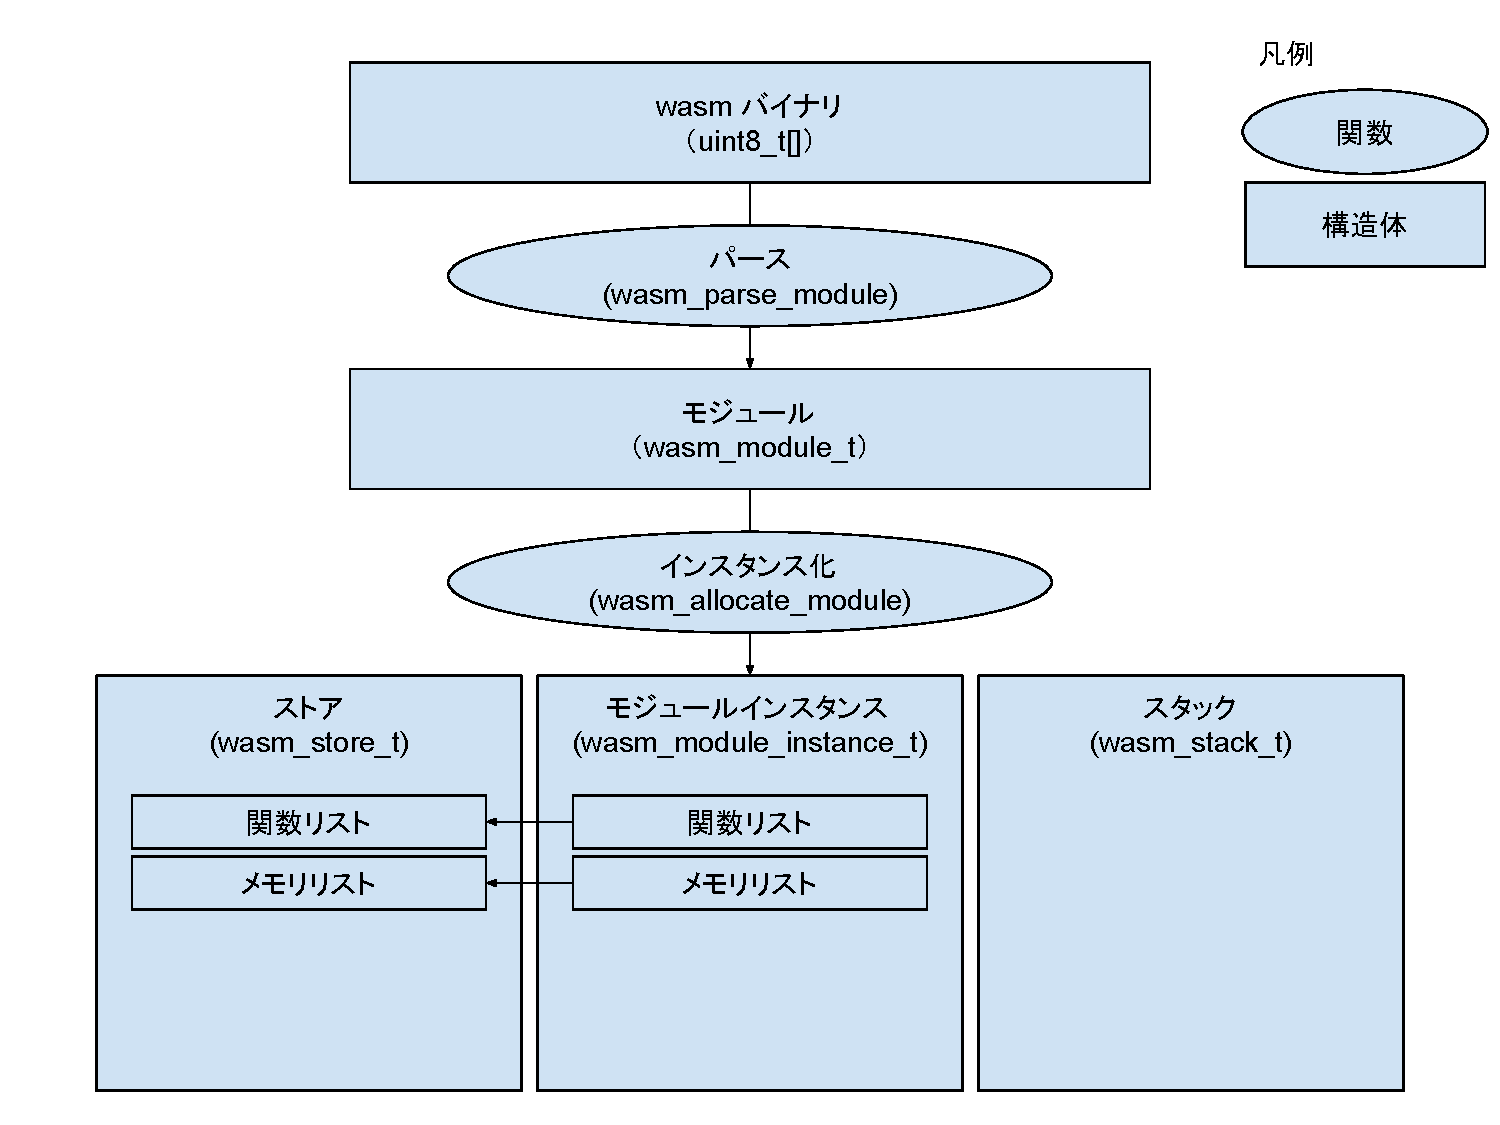
\includegraphics[bb=0 0 960 720,width=12cm]{img/libwasm_arch.pdf}
  \end{center}
\end{figure}

libwasmにおける実行環境は、各WebAssemblyモジュールの情報を格納するストア(\verb|wasm_store_t|)と、
演算対象となるスタック(\verb|wasm_stack_t|)から成る。

libwasmを用いてWebAssemblyプログラムを実行するには、まずWebAssemblyバイナリ(バイト列)を
\verb|wasm_parse_module|関数によりパースし、WebAssemblyモジュール(\verb|wasm_module_t|)を得る。

次に、WebAssemblyモジュールの情報を\verb|wasm_allocate_module|関数によりストアに読み込む(アロケーション)。
これにより、当該モジュール内の関数が呼び出し可能になる。
\verb|wasm_allocate_module|関数はアロケーションの結果としてモジュールインスタンス
(\verb|wasm_module_instance_t|)を返す。
モジュールインスタンスは、モジュールの関数やメモリの参照(アドレス)だけを保持し、実態はストア内に保持される。
ストアは読み込んだ全てのモジュールの関数やメモリのデータを一括して保持するため、
あるモジュールが他のモジュールの関数やメモリを参照することが可能となる。

スタックには、演算対象となる値、制御命令の適用範囲を示すラベル、そして関数呼び出しの情報を格納するアクティベーションが格納される。
WebAssembly実行環境において、スタックはpopまたはpushによってしか操作されず、線形にアクセスされることはない。
そのためlibwasmでは、スタックをヒープ領域上の線形リストとして実装した。
